%Copyright 2014 Jean-Philippe Eisenbarth
%This program is free software: you can 
%redistribute it and/or modify it under the terms of the GNU General Public 
%License as published by the Free Software Foundation, either version 3 of the 
%License, or (at your option) any later version.
%This program is distributed in the hope that it will be useful,but WITHOUT ANY 
%WARRANTY; without even the implied warranty of MERCHANTABILITY or FITNESS FOR A 
%PARTICULAR PURPOSE. See the GNU General Public License for more details.
%You should have received a copy of the GNU General Public License along with 
%this program.  If not, see <http://www.gnu.org/licenses/>.

%Based on the code of Yiannis Lazarides
%http://tex.stackexchange.com/questions/42602/software-requirements-specification-with-latex
%http://tex.stackexchange.com/users/963/yiannis-lazarides
%Also based on the template of Karl E. Wiegers
%http://www.se.rit.edu/~emad/teaching/slides/srs_template_sep14.pdf
%http://karlwiegers.com
\documentclass{scrreprt}
\usepackage{listings}
\usepackage{amsmath}
\usepackage{underscore}
\usepackage{multicol}
\usepackage{tikz}
\usetikzlibrary{positioning}
\usepackage{standalone}
\usepackage[bookmarks=true]{hyperref}
\usepackage[utf8]{inputenc}
\usepackage[english]{babel}
\hypersetup{
    bookmarks=false,    % show bookmarks bar?
    pdftitle={Software Requirement Specification},    % title
    pdfauthor={Jean-Philippe Eisenbarth},                     % author
    pdfsubject={TeX and LaTeX},                        % subject of the document
    pdfkeywords={TeX, LaTeX, graphics, images}, % list of keywords
    colorlinks=true,       % false: boxed links; true: colored links
    linkcolor=blue,       % color of internal links
    citecolor=black,       % color of links to bibliography
    filecolor=black,        % color of file links
    urlcolor=purple,        % color of external links
    linktoc=page            % only page is linked
}%
\def\myversion{1.0 }
\date{}
%\title
\usepackage{hyperref}
\begin{document}

\begin{flushright}
    \rule{16cm}{5pt}\vskip1cm
    \begin{bfseries}
        \Huge{SOFTWARE REQUIREMENTS\\ SPECIFICATION}\\
        \vspace{1cm}
        for\\
        \vspace{1cm}
        Attendance Application\\
        \vspace{1cm}
        \LARGE{Version \myversion approved}\\
        \vspace{0cm}
        \begin{align*}
        \text{Prepared by: } \;\;\;\; 
         &\text{Sanskar Mittal} &\text{21CS10057}\\
         &\text{Yash Sirvi} &\text{21CS10083}\\
         &\text{Ashwin Prasanth} &\text{21CS30009}\\
        \end{align*}
        \vspace{1.9cm}
        Indian Institute of Technology Kharagpur\\
        \vspace{1.9cm}
        \today\\
    \end{bfseries}
\end{flushright}

\tableofcontents


% \chapter*{Revision History}

% \begin{center}
%     \begin{tabular}{|c|c|c|c|}
%         \hline
% 	    Name & Date & Reason For Changes & Version\\
%         \hline
% 	    21 & 22 & 23 & 24\\
%         \hline
% 	    31 & 32 & 33 & 34\\
%         \hline
%     \end{tabular}
% \end{center}

\chapter{Introduction}

\section{Purpose}
The purpose of this document is to define the software requirements for the development of an Attendance Application. This software is intended to be used by educational institutions, businesses, and organizations to track the attendance of students, employees, or members. The application will be designed to provide a user-friendly interface, allowing easy and efficient management of attendance records.

The Attendance Application will be developed to provide an automated system that simplifies the attendance-taking process. The software will be designed to reduce the workload of teachers, administrators, and human resource personnel who are responsible for tracking attendance.

This document will outline the functional and non-functional requirements of the software, including the user interface.

% \section{Document Conventions}
% $<$Describe any standards or typographical conventions that were followed when 
% writing this SRS, such as fonts or highlighting that have special significance.  
% For example, state whether priorities  for higher-level requirements are assumed 
% to be inherited by detailed requirements, or whether every requirement statement 
% is to have its own priority.$>$

\section{Intended Audience and Reading Suggestions}
    % \vspace*{-4pt}
This document is intended for the following audience:
    % \vspace*{-7pt}
\begin{itemize}
    \item The development team responsible for implementing the Attendance Application software
    % \vspace*{-7pt}
    \item System administrators and users who will be responsible for installing and using the Attendance Application software
    % \vspace*{-7pt}
    \item Any other parties involved in the development, testing, and deployment of the Attendance Application software
\end{itemize}

    % \vspace*{-7pt}
To fully understand the requirements and constraints outlined in this document, it is recommended that readers have a working knowledge of the following:
    % \vspace*{-7pt}

\begin{itemize}
    \item Object-oriented programming concepts and practices
    % \vspace*{-7pt}
    \item Android application development technologies and tools such as Android Studio and React Native
    % \vspace*{-7pt}
    \item Relational database management systems and SQL
\end{itemize}

To read the document, readers should start with the Overview sections, including the Introduction and Overall Description,
 to gain a high-level understanding of the Attendance Application software and its purpose. From there, readers can move on to the sections 
 that are most pertinent to their specific role or area of responsibility, such as the Other Nonfunctional Requirements section for developers,
  the External Interface Requirements section for project managers and testers. 

\section{Project Scope}
The Attendance Application software is designed to provide an efficient and reliable way for educational institutions to track student attendance. The system is intended to be used by both students and faculty, with different roles and permissions assigned to each user type.

The Attendance Application software will be designed as a smartphone-based application that can be accessed by both students and faculty using their mobile devices. The system will be developed using industry-standard technologies and will be scalable to accommodate additional users and institutions as needed.

% \section{References}
% $<$List any other documents or Web addresses to which this SRS refers. These may 
% include user interface style guides, contracts, standards, system requirements 
% specifications, use case documents, or a vision and scope document. Provide 
% enough information so that the reader could access a copy of each reference, 
% including title, author, version number, date, and source or location.$>$


\chapter{Overall Description}

\section{Product Perspective}
The Attendance Application software is a new, self-contained product that is being developed to provide an efficient and reliable way for educational institutions to track student attendance. The system will be designed as a smartphone-based application that can be accessed by both students and faculty using their mobile devices.


\section{Product Functions}
The Attendance Application software will include the following features and functionality:
\begin{multicols}{2}
    \begin{itemize}
        \item Student attendance tracking
        \vspace{-4pt}
        \item Attendance reports
        \vspace{-4pt}
        \item Notification system
        \vspace{-4pt}
        \item User authentication and security
        \vspace{-4pt}
        \item Proxy Detection
        \vspace{-4pt}
        \item Importing and Exporting data
    \end{itemize}
\end{multicols}

% $<$Summarize the major functions the product must perform or must let the user 
% perform. Details will be provided in Section 3, so only a high level summary 
% (such as a bullet list) is needed here. Organize the functions to make them 
% understandable to any reader of the SRS. A picture of the major groups of 
% related requirements and how they relate, such as a top level data flow diagram 
% or object class diagram, is often effective.$>$

\section{User Classes and Characteristics}
\begin{enumerate}
    \item \textbf{administrator} $-$ The administrator is responsible for managing the attendance records of students and faculty. The administrator will be able to view attendance records and manage user accounts.
    \item \textbf{teacher} $-$ The teacher is responsible for creating courses and editing attendance records for students in their courses. The teacher will be able to view attendance records and generate attendance reports.
    \item \textbf{student} $-$ The student is responsible for marking their own attendance. The student will be able to view their own attendance records and generate attendance reports. 
\end{enumerate}
% $<$Identify the various user classes that you anticipate will use this product.  
% User classes may be differentiated based on frequency of use, subset of product 
% functions used, technical expertise, security or privilege levels, educational 
% level, or experience. Describe the pertinent characteristics of each user class.  
% Certain requirements may pertain only to certain user classes. Distinguish the 
% most important user classes for this product from those who are less important 
% to satisfy.$>$

\section{Operating Environment}
The Attendance Application software will be designed to operate on mobile devices running Android 7.0 and above, as well as iOS 11 and above.

The software components and applications that need to peacefully coexist with the Attendance Application software are: Web server, Database system, and Network infrastructure
Overall, the Attendance Application software will operate in a networked environment that requires the peaceful coexistence of multiple software components and applications.


\section{Design and Implementation Constraints}
\subsection{Use-Case Diagram}
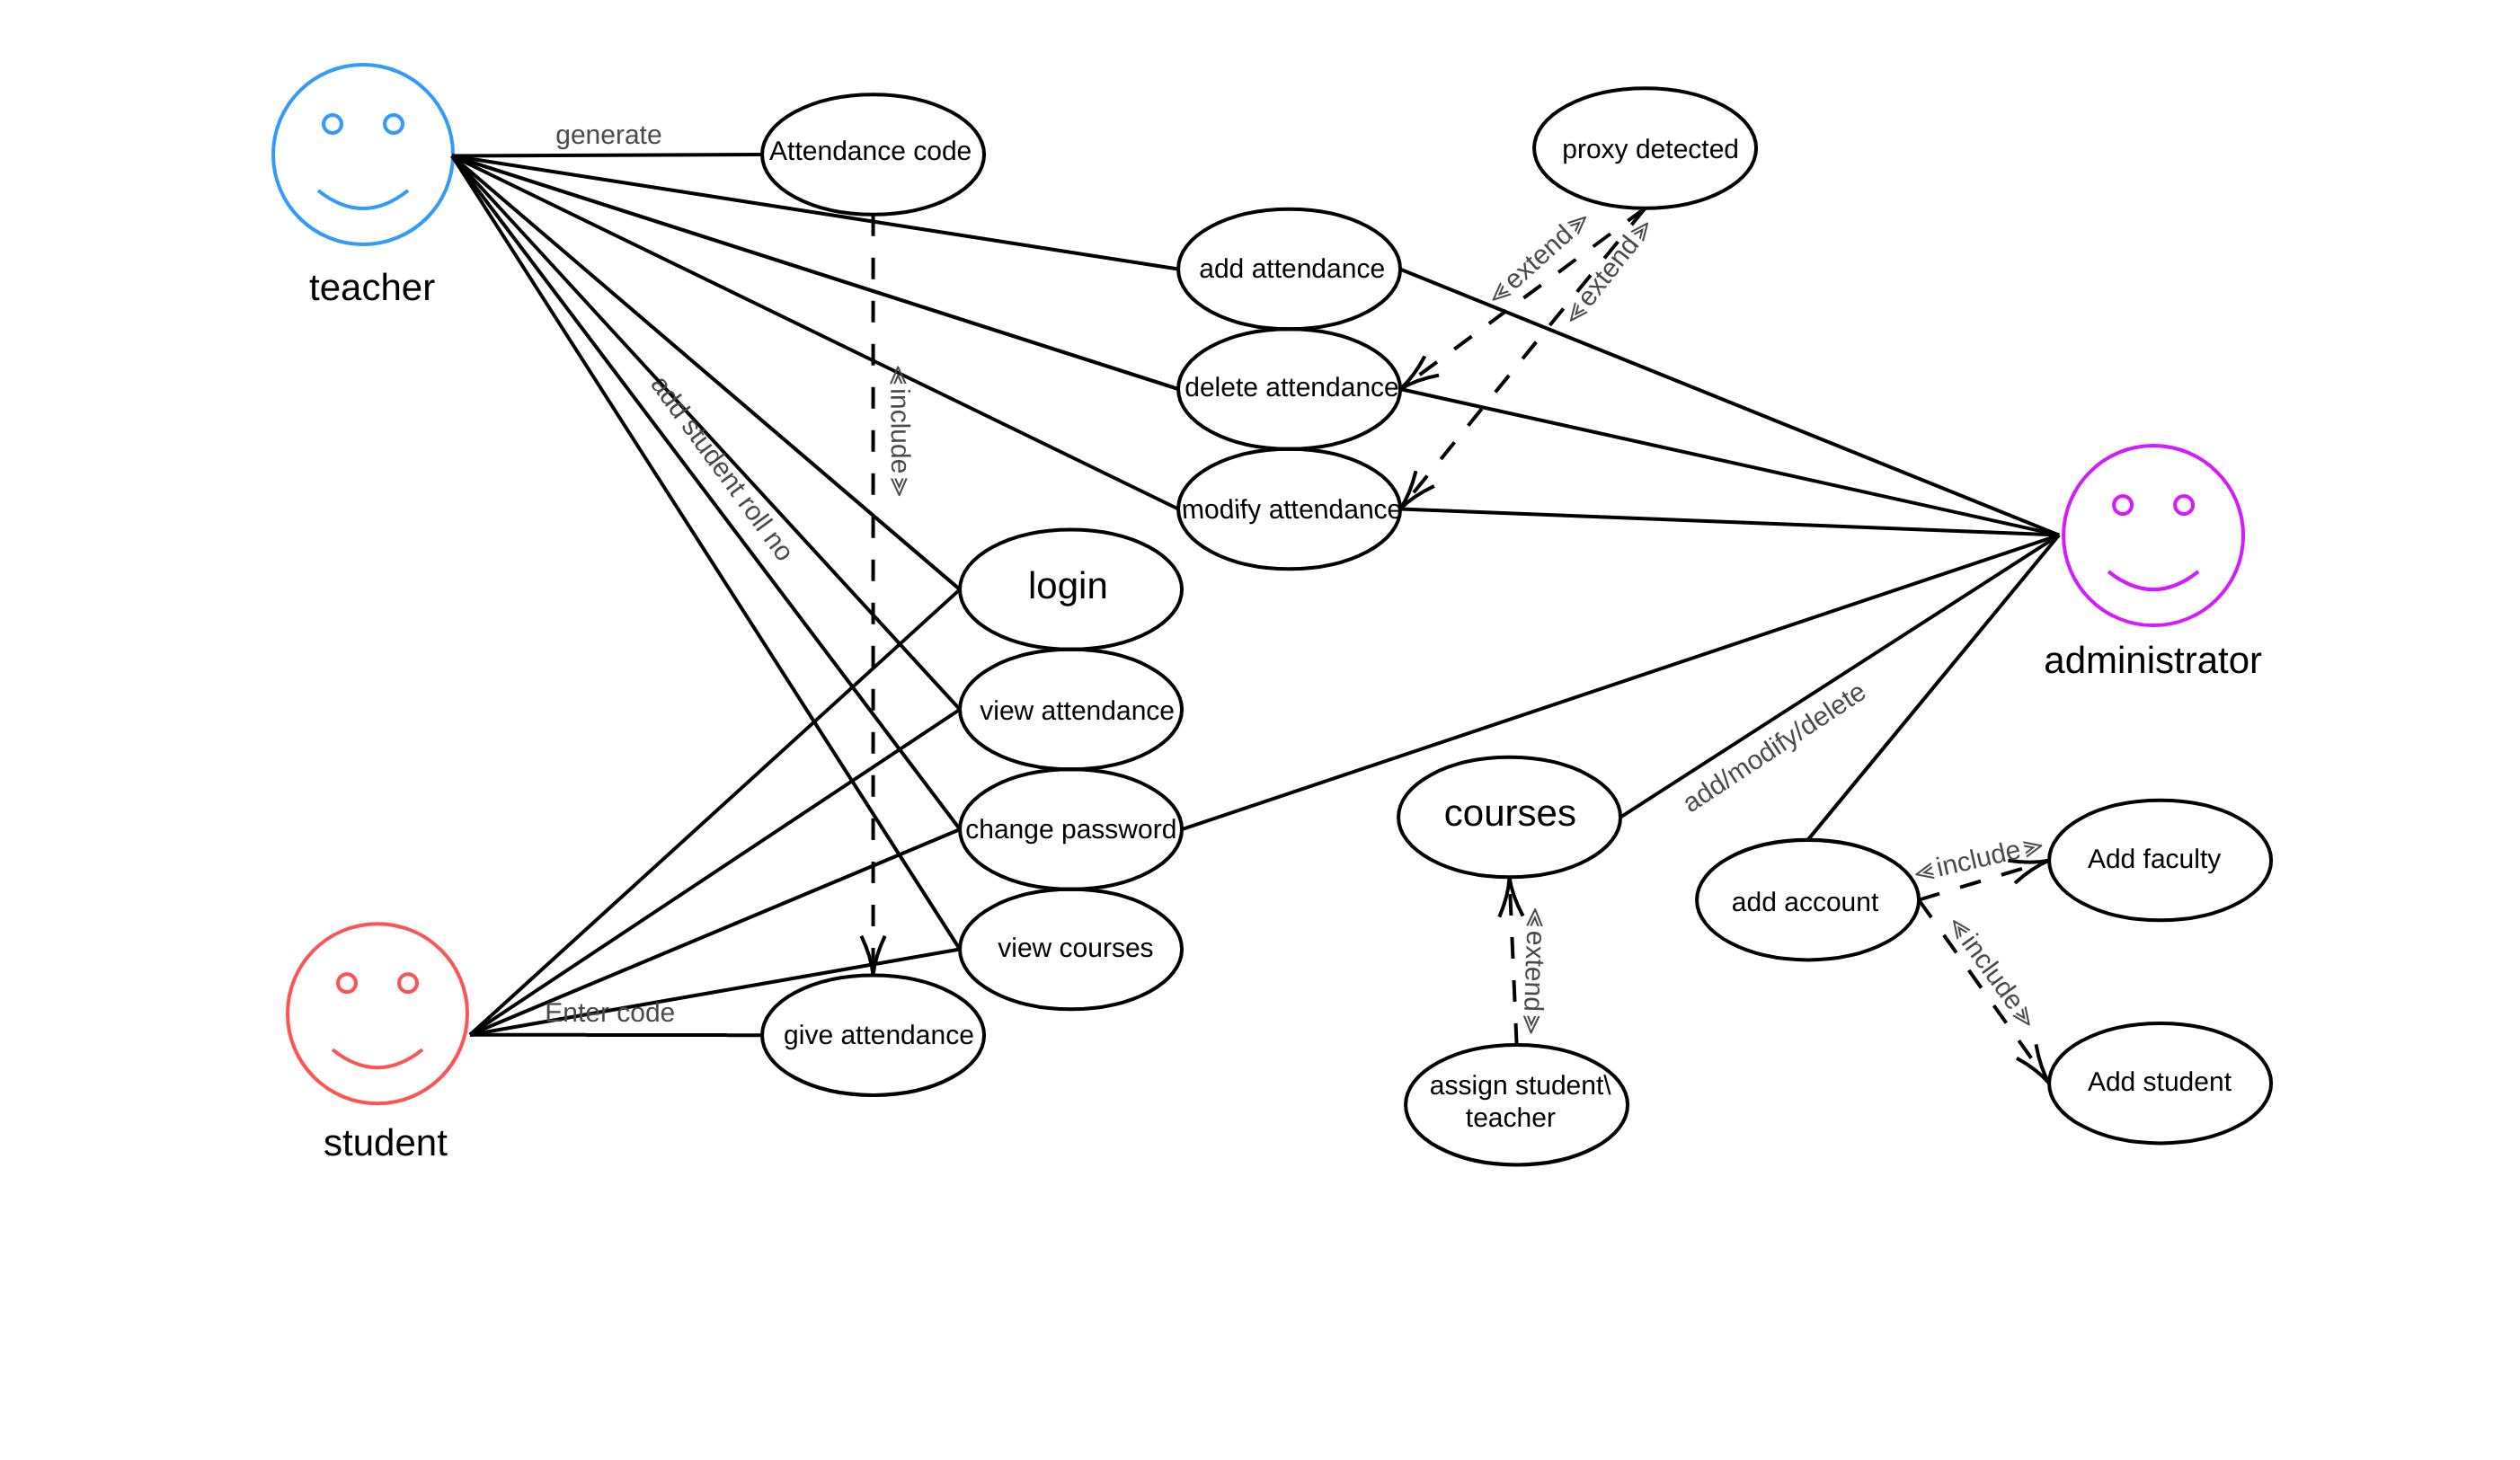
\includegraphics[width=\linewidth]{use-case.png}
\subsection{Class Diagram}
\includegraphics[width=\linewidth]{"class diagram.png"}
\subsection{Constraints}
The development of the Attendance Application software is subject to the following constraints:
\begin{itemize}
\item Limited time: The development team has a fixed short timeline for completing the
project.
\item Learning new frameworks: The development team will need to learn and use new
frameworks to develop the app. This requires
additional time and resources to ensure the team has the necessary skills.
\item Security considerations: The Attendance Application software will handle sensitive data, including student and course information. Security considerations will need to be considered during the design and development phases.
\end{itemize}

\section{User Documentation}
The Attendance Application software will be accompanied by a user documentation package that will include the following materials:
\begin{itemize}
\item User manual: User manual including step-by-step instructions will be provided to guide users through
installing and using the software.
\item Quick reference guide: A quick reference guide will be provided to help users
perform common tasks, such as taking attendance or generating and exporting reports.
\item Relevant technology documentation: The user documentation package will also
include links to relevant technical documentation, such as React Native docu-
mentation.
\end{itemize}


\chapter{External Interface Requirements}

\section{User Interfaces}
\subsection{Home Page} 
It gives 3 options for login - for student, teacher or design
It also gives an additional option for new users to register 

\subsection{Login/Register Page}
In this page, Login/Registration is done by taking relevant input from user (E-mail ID, Password, and some additional information in case of Registration). 
Moreover, it will show an option of "Forgot Password" in Login 

\subsection{Student Home Page}
This will show an option at the top to give attendance, if a course is going on currently and attendance period is active. 
 Below that, a list of the student's currently enrolled course would be visible. 
On clicking on a certain course, it gives them a record of their attendance in that course. 

\subsection{Teacher Home Page}
This will show an option to take attendance, if a class is going on, and an option to close attendance period if it is currently open.
Below it is a list of the Teacher's current courses. On clicking on any of them, it gives the Teacher a student-wise record of attendance along with overall statistics. 

\subsection{Admin Home Page}
This will show the admin a list of courses, and an option to edit or add courses at the top. On clicking of any of the courses, they get an option to modify teacher, add/remove student and modify student attendance.
% $<$Describe the logical characteristics of each interface between the software 
% product and the users. This may include sample screen images, any GUI standards 
% or product family style guides that are to be followed, screen layout 
% constraints, standard buttons and functions (e.g., help) that will appear on 
% every screen, keyboard shortcuts, error message display standards, and so on.  
% Define the software components for which a user interface is needed. Details of 
% the user interface design should be documented in a separate user interface 
% specification.$>$

% \section{Hardware Interfaces}
% $<$Describe the logical and physical characteristics of each interface between 
% the software product and the hardware components of the system. This may include 
% the supported device types, the nature of the data and control interactions 
% between the software and the hardware, and communication protocols to be 
% used.$>$

\section{Software Interfaces}
The system will be made to function on both Android and iOS. Both the student and the teacher are supposed to use smartphones with location-sharing capabilities via GPRS. This will aid in the proxy detection during attendance.

% \section{Communications Interfaces}
% $<$Describe the requirements associated with any communications functions 
% required by this product, including e-mail, web browser, network server 
% communications protocols, electronic forms, and so on. Define any pertinent 
% message formatting. Identify any communication standards that will be used, such 
% as FTP or HTTP. Specify any communication security or encryption issues, data 
% transfer rates, and synchronization mechanisms.$>$


\chapter{System Features}
% $<$This template illustrates organizing the functional requirements for the 
% product by system features, the major services provided by the product. You may 
% prefer to organize this section by use case, mode of operation, user class, 
% object class, functional hierarchy, or combinations of these, whatever makes the 
% most logical sense for your product.$>$

\section{Student Attendance Tracking}


\subsection{Description and Priority}
Priority: \textbf{High}

This feature allows teachers and instructors to keep track of student attendance in real-time.
The feature enables teachers to create and manage courses, and edit attendance for each student.
Students can also view their attendance record, including their current attendance percentage, the number of days present, absent, and late.
% \subsection{Stimulus/Response Sequences}
% $<$List the sequences of user actions and system responses that stimulate the 
% behavior defined for this feature. These will correspond to the dialog elements 
% associated with use cases.$>$

\subsection{Functional Requirements}
\begin{itemize}
    \item REQ-1: The system shall allow teachers to create and manage courses.
    \item REQ-2: The system shall allow teachers to edit attendance for each student.
    \item REQ-3: The system shall allow students to enroll in courses set up by teachers. 
    \item REQ-4: The system shall allow students to mark their attendance within a specified time frame for each course.
    \item REQ-5: The system shall allow students to view their attendance records.
\end{itemize}
% $<$Itemize the detailed functional requirements associated with this feature.  
% These are the software capabilities that must be present in order for the user 
% to carry out the services provided by the feature, or to execute the use case.  
% Include how the product should respond to anticipated error conditions or 
% invalid inputs. Requirements should be concise, complete, unambiguous, 
% verifiable, and necessary. Use “TBD” as a placeholder to indicate when necessary 
% information is not yet available.$>$

% $<$Each requirement should be uniquely identified with a sequence number or a 
% meaningful tag of some kind.$>$

% REQ-1:	REQ-2:

\section{User Authentication}
\subsection{Description and Priority}
Priority: \textbf{High}

This feature allows users to create an account and log in to the app. The allowed user types are students, teachers, and administrators. 
Only administrators can accept new user account creation requests.
% \subsection{Stimulus/Response Sequences}
% $<$List the sequences of user actions and system responses that stimulate the 
% behavior defined for this feature. These will correspond to the dialog elements 
% associated with use cases.$>$

\subsection{Functional Requirements}
\begin{itemize}
    \item REQ-1: The system shall allow users to create an account in categories of student, teacher, or administrator.
    \item REQ-2: The system shall allow users to log in to the app using correct credentials.
    \item REQ-3: The system shall allow only administrators to accept new user account creation requests.
\end{itemize}


\section{Attendance Reports}
\subsection{Description and Priority}
Priority: \textbf{Medium}

This feature allows teachers and students to view attendance reports for each course. Teachers can view attendance reports for all students in a course, while students can view their own attendance reports.
% \subsection{Stimulus/Response Sequences}
% $<$List the sequences of user actions and system responses that stimulate the 
% behavior defined for this feature. These will correspond to the dialog elements 
% associated with use cases.$>$

\subsection{Functional Requirements}
\begin{itemize}
    \item REQ-1: The system shall create attendance reports for each student in each course.
    \item REQ-2: The system shall allow teachers to view attendance reports for all students in a course.
    \item REQ-3: The system shall allow students to view their own attendance reports.
\end{itemize}


\section{Proxy Detection}
\subsection{Description and Priority}
Priority: \textbf{Medium}

This feature allows teachers to detect students who are using a proxy to mark their attendance.
% \subsection{Stimulus/Response Sequences}
% $<$List the sequences of user actions and system responses that stimulate the 
% behavior defined for this feature. These will correspond to the dialog elements 
% associated with use cases.$>$

\subsection{Functional Requirements}
\begin{itemize}
    \item REQ-1: The system should detect students who are using a proxy to mark their attendance.
\end{itemize}

\section{Notification System}
\subsection{Description and Priority}
Priority: \textbf{Low}

This feature allows teachers to send notifications to students regarding low or irregular attendance to any student in a course.
% \subsection{Stimulus/Response Sequences}
% $<$List the sequences of user actions and system responses that stimulate the 
% behavior defined for this feature. These will correspond to the dialog elements 
% associated with use cases.$>$

\subsection{Functional Requirements}
\begin{itemize}
    \item REQ-1: System should be able to notify students.
\item REQ-2: System should allow teachers to modify and send notifications to students.
\end{itemize}

\section{Importing and Exporting Data}
\subsection{Description and Priority}
Priority: \textbf{Low}

This feature should allow teachers and administrators to import and export data from the system.
This will allow already existing data to be imported into the system, and data from the system to be exported to other systems.
% \subsection{Stimulus/Response Sequences}
% $<$List the sequences of user actions and system responses that stimulate the 
% behavior defined for this feature. These will correspond to the dialog elements 
% associated with use cases.$>$

\subsection{Functional Requirements}
\begin{itemize}
    \item REQ-1: System should work with CSV files to store data.
    \item REQ-2: System should allow teachers and administrators to import and export data from the system.
\end{itemize}


\chapter{Other Nonfunctional Requirements}

% \section{Performance Requirements}
% $<$If there are performance requirements for the product under various 
% circumstances, state them here and explain their rationale, to help the 
% developers understand the intent and make suitable design choices. Specify the 
% timing relationships for real time systems. Make such requirements as specific 
% as possible. You may need to state performance requirements for individual 
% functional requirements or features.$>$

\section{Safety Requirements}

\begin{itemize}
    \item The system will store sensitive information essential to the functioning of Institutions which will be using it.
        It is therefore essential to keep backups of everything and to ensure that the data is not lost.
    \item The system will be used by students and teachers who are not necessarily tech-savvy.
        It is therefore essential to ensure that the system is easy to use and does not require any special training.
    \item The system should also be able to handle any errors that may occur.
    \item The system should expect the proxy detection to not be perfect and should be able to handle false positives.

\end{itemize}

% $<$Specify those requirements that are concerned with possible loss, damage, or 
% harm that could result from the use of the product. Define any safeguards or 
% actions that must be taken, as well as actions that must be prevented. Refer to 
% any external policies or regulations that state safety issues that affect the 
% product’s design or use. Define any safety certifications that must be 
% satisfied.$>$

\section{Security Requirements}
\begin{itemize}
    \item The system will handle sensitive information such as student and teacher details.
        It is therefore essential to ensure that the system is secure and that the data is not leaked.
    \item The login feature should not be vulnerable to brute force attacks.
    \item The import and export feature should not be vulnerable to SQL injection attacks.
\end{itemize}

% $<$Specify any requirements regarding security or privacy issues surrounding use 
% of the product or protection of the data used or created by the product. Define 
% any user identity authentication requirements. Refer to any external policies or 
% regulations containing security issues that affect the product. Define any 
% security or privacy certifications that must be satisfied.$>$

\section{Software Quality Attributes}
The following are the quality attributes that the system should have from highest to lowest priority:
\begin{itemize}
    \item The application should not be platform dependent and should be able to run on both Android and IOS devices.
    \item The system should be easy to use as it will be used by students and teachers who are not necessarily tech-savvy.
    \item The codebase should be well documented and easy to understand. This will allow for easier maintenance and addition of new features.
    \item The application should be able to handle any errors that may occur.
    \item The application should be lightweight and fast to use.
\end{itemize}
% $<$Specify any additional quality characteristics for the product that will be 
% important to either the customers or the developers. Some to consider are: 
% adaptability, availability, correctness, flexibility, interoperability, 
% maintainability, portability, reliability, reusability, robustness, testability, 
% and usability. Write these to be specific, quantitative, and verifiable when 
% possible. At the least, clarify the relative preferences for various attributes, 
% such as ease of use over ease of learning.$>$

% \section{Business Rules}
% $<$List any operating principles about the product, such as which individuals or 
% roles can perform which functions under specific circumstances. These are not 
% functional requirements in themselves, but they may imply certain functional 
% requirements to enforce the rules.$>$


% \chapter{Other Requirements}
% $<$Define any other requirements not covered elsewhere in the SRS. This might 
% include database requirements, internationalization requirements, legal 
% requirements, reuse objectives for the project, and so on. Add any new sections 
% that are pertinent to the project.$>$

% \section{Appendix A: Glossary}
% %see https://en.wikibooks.org/wiki/LaTeX/Glossary
% $<$Define all the terms necessary to properly interpret the SRS, including 
% acronyms and abbreviations. You may wish to build a separate glossary that spans 
% multiple projects or the entire organization, and just include terms specific to 
% a single project in each SRS.$>$

% \section{Appendix B: Analysis Models}
% $<$Optionally, include any pertinent analysis models, such as data flow 
% diagrams, class diagrams, state-transition diagrams, or entity-relationship 
% diagrams.$>$

% \section{Appendix C: To Be Determined List}
% $<$Collect a numbered list of the TBD (to be determined) references that remain 
% in the SRS so they can be tracked to closure.$>$

\end{document}
